\documentclass[a3, landscape]{a0poster}
\usepackage{graphicx,lipsum}
\usepackage[paperwidth=297mm,paperheight=420mm,margin=0mm, landscape]{geometry}
\usepackage{calc}
\pagestyle{empty}
\usepackage{xcolor}
\usepackage{psfrag}
\usepackage{pstricks,pst-node,pstricks-add, pst-text}
\DeclareFixedFont{\RM}{T1}{ptm}{b}{n}{2cm}
\definecolor{oxblue}{cmyk}{1,0.8,0,0.6}
%\definecolor{oxblue}{RGB}{0,33,71}
\definecolor{yell}{cmyk}{0.04,0.16,0.84,0}
\definecolor{yell2}{cmyk}{0.16,0.59,0.96,0.02}
\usepackage[space]{grffile} % for spaces in file names?
\renewcommand{\labelitemi}{${\color{yell2}\bullet}$}
\usepackage{lmodern}
\usepackage{xcolor}

\usepackage{natbib}
\usepackage[hyphens]{url}
\usepackage[hidelinks]{hyperref}
\hypersetup{breaklinks=true}
\usepackage[hyphenbreaks]{breakurl}
\setlength{\bibsep}{0pt plus 0.3ex}
\hypersetup{
    colorlinks,
    linkcolor={red!50!black},
    citecolor={blue!80!black},
    urlcolor={blue!90!black}
}
\DeclareRobustCommand{\firstsecond}[2]{#1}
\makeatletter
  \newcommand{\miniscule}{\@setfontsize\miniscule{5}{6}}% \tiny: 5/6
    \newcommand{\minisculey}{\@setfontsize\minisculey{6}{7}}% \tiny: 5/6
  \newcommand{\mini}{\@setfontsize\miniscule{8}{9}}% \tiny: 5/6
  \newcommand{\maxi}{\@setfontsize\miniscule{10}{11}}% \tiny: 5/6
  \newcommand{\BBB}{\@setfontsize\BBB{32}{33}}% \tiny: 5/6

\makeatother


\begin{document}


\noindent\begin{pspicture}[showgrid=true](\paperwidth, \paperheight)
\psline(0.5,41.3)(29.2,41.3)
\psline(0.5,39.5)(29.2,39.5)
\rput[bl](0.5,39.6){\BBB  Household Living Arrangements of Elderly People}
\psline(0.5,1.2)(29.2,1.2)
\rput[bl](0.5,0.3){\small\textsc{Population Horizons Factsheet IV.} 
\scriptsize (2016) Vol.13 Issue 2}


\rput[br](29.2,39.7){
\includegraphics[height=1.4cm]{../figures/dglogo}}

\rput[br](29.2,0.05){
\minisculey \emph{Prepared by Maja Zalo\v znik} -- DOI XXXXXX -- S.3}
%
\rput[tl](0.5,38.9){
\rput[tl](0,0.2){
\mini{\parbox[c]
{13.5cm}{
\footnotesize \textsc{Proportions of people over 60 by household type and intergenerational living arrangements in selected countries}

\vspace{1ex}
\maxi Using census microdata collected by IPUMS (XX) we summarise the types of households in which the elderly (over 60 years old) live. We use two typologies:
 \begin{itemize}
 \item Household composition based on kinship XX
 \item Intergenerational household type
\end{itemize}  
}}}
}
%
%\rput[bl](0.5,19.18571){
%
%\rput[bl](0,0.2){
%\mini{\parbox[c]
%{13.5cm}{\maxi The population growth rates are taken from the World Bank Development Indicators \citep{2017wb} and refer to the annual growth of the number of residents in a country. The fertility rates are from the UN World Fertility Data \citep{2015un} which compiles data and estimates from numerous sources, both registration and survey based calculations, hence the large number of data points in some cases.  
%}}}
%}
%
%
%\rput[bl](0.5,12){
%\rput[bl](0,0.2){
%\mini{\parbox[c]
%{13.5cm}{\maxi The United Nations \citep{2015unb} records countries' population policies as \emph{``the government's policy to influence the rate of population growth or the level of fertility in the country''}. Reporting started in 1976; however, long breaks in between the early reports do not necessarily mean the policies remained the same throughout the whole period so the early sections should be interpreted with care. 
%}}}
%}




%\rput[bl](15,6.3){
%\rput[bl](0,0.2){
%\mini{\parbox[c]
%{14cm}{\maxi \Urlmuskip=0mu plus 1mu\relax
%\bibliographystyle{apa}
%\renewcommand\refname{}
%\vspace*{-2cm}
%\mini{\bibliography{lit.bib}} 
%}}}
%}


%% 1,1
\psfrag{A}[c][c]{\miniscule{Men}}
\psfrag{B}[c][c]{\miniscule{Women}}
\psfrag{1}[r][c]{\miniscule{\emph{Single}}}
\psfrag{2}[r][c]{\miniscule{\emph{Nuclear}}}
\psfrag{3}[r][c]{\miniscule{\emph{Extended}}}
\psfrag{4}[r][c]{\miniscule{\emph{Complex}}}

\psfrag{5}[c][c]{\miniscule{0}}
\psfrag{6}[c][c]{\miniscule{0.2}}
\psfrag{7}[c][c]{\miniscule{0.4}}
\psfrag{8}[c][c]{\miniscule{0.6}}
\psfrag{9}[c][c]{\miniscule{0.8}}
\psfrag{0}[c][c]{\miniscule{1}}


\psfrag{a}[l][c]{\miniscule{\emph{Single}}}
\psfrag{b}[l][c]{\miniscule{\emph{One gen.}}}
\psfrag{c}[l][c]{\miniscule{\emph{Two gen.}}}
\psfrag{d}[l][c]{\miniscule{\emph{Three+ gen.}}}
\psfrag{e}[l][c]{\miniscule{\emph{Skipped gen.}}}

\rput[bl](0,1.5){

\psset{xunit=7.425cm, yunit=4.7cm}
% 1,1
\rput[bl](0,0){
\rput[bl](0,0){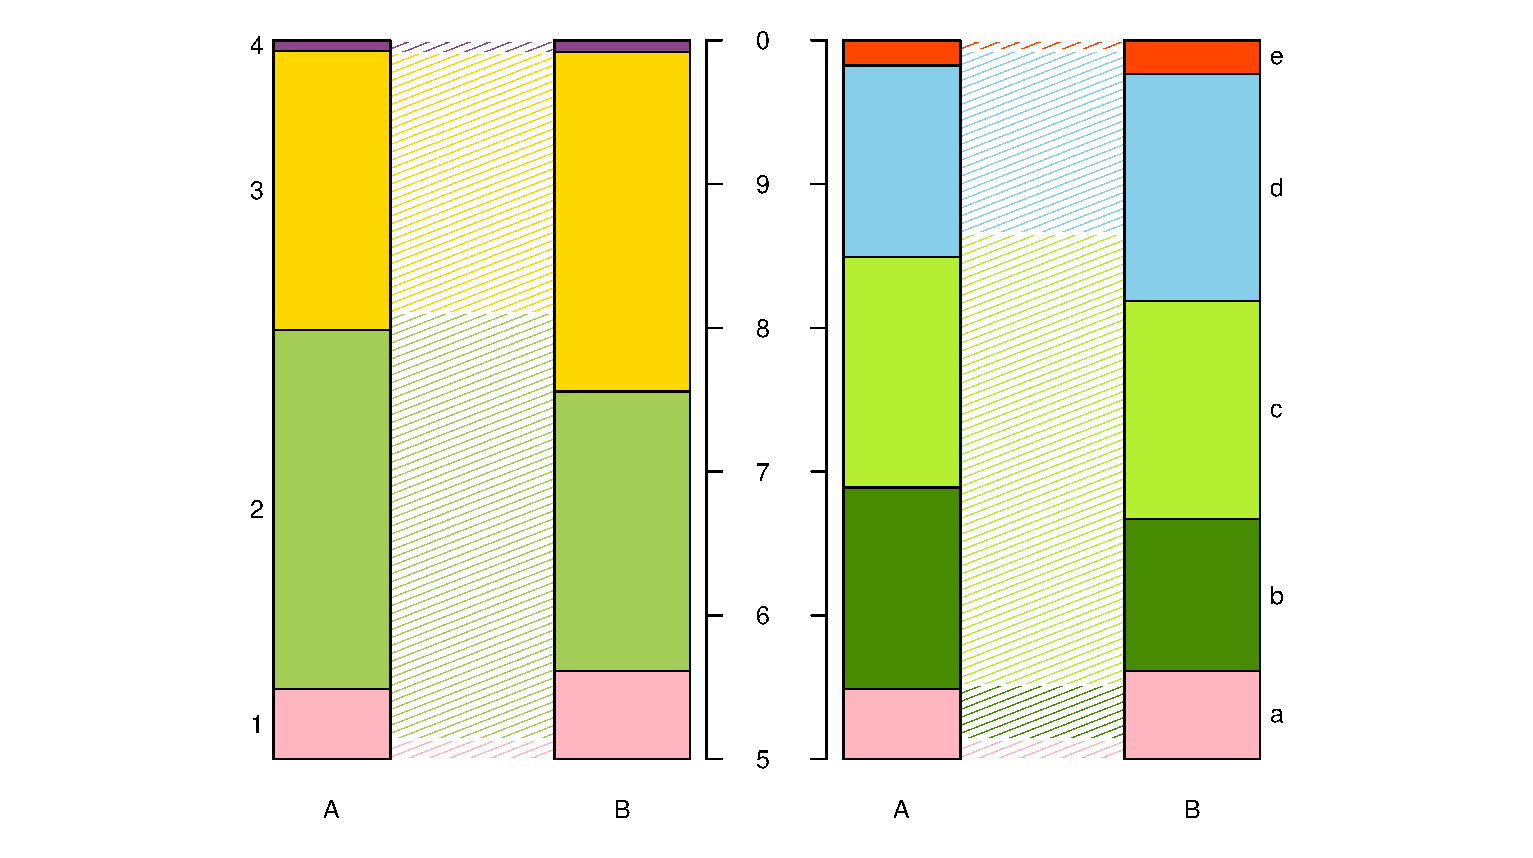
\includegraphics[width=7.425cm]{../figures/Mexico}}
\rput[bl](0.05,0.88) {\footnotesize  Mexico (2015)}
%\psframe(0,0)(1,1)
}

\rput[bl](0.05,2.1){\large \textsc{Americas}
}
% 1,2
\rput[bl](0,1){
\rput[bl](0,0){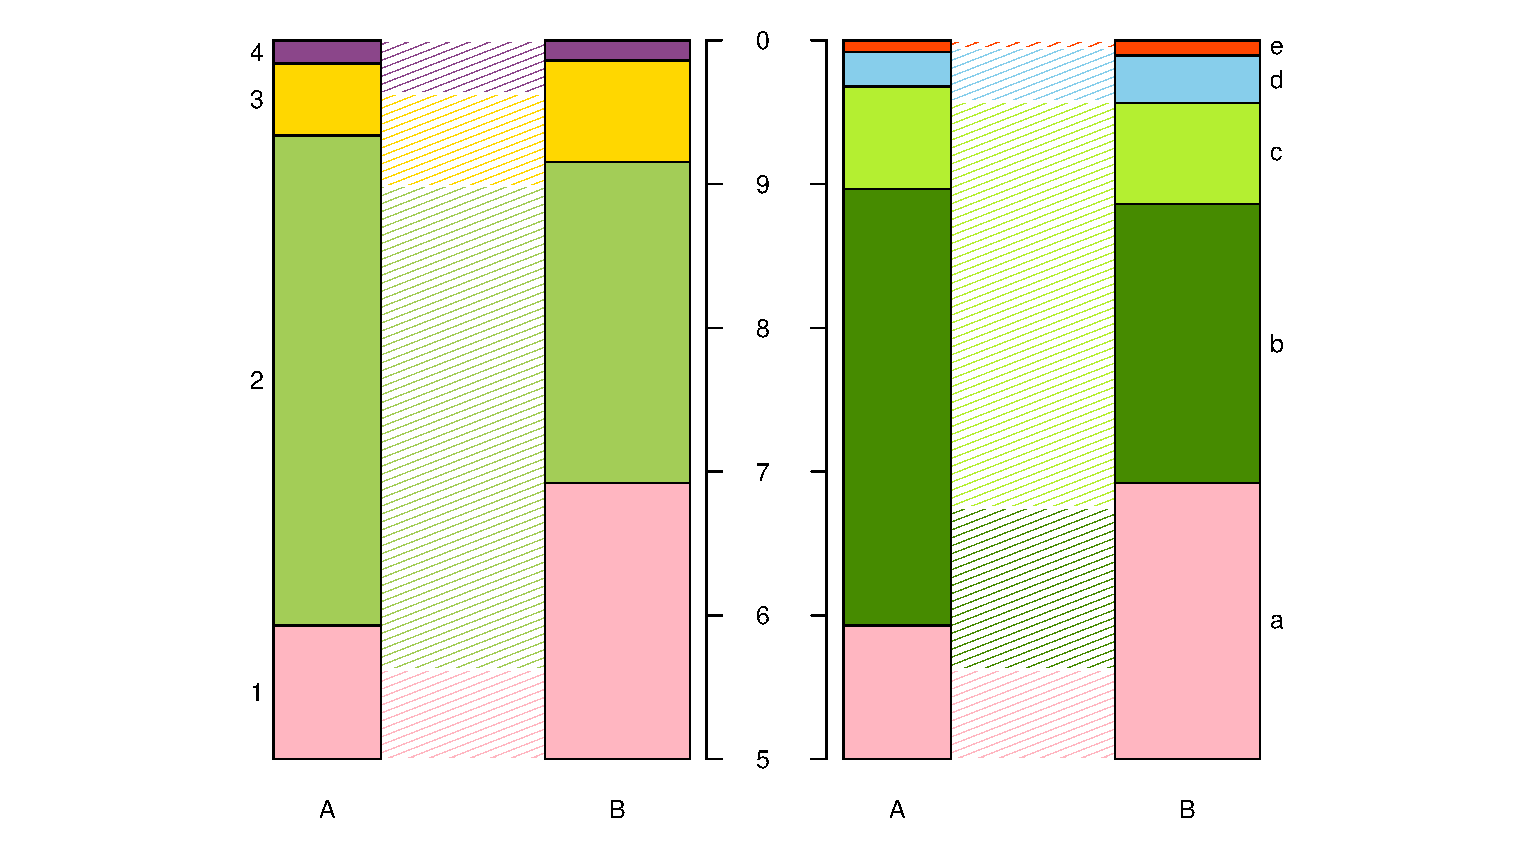
\includegraphics[width=7.425cm]{../figures/UnitedStates}}
\rput[bl](0.05,0.85) {\footnotesize United States (2000)}
%\psframe(0,0)(1,1)
}

% 2,1
\rput[bl](1,0){
\rput[bl](0,0){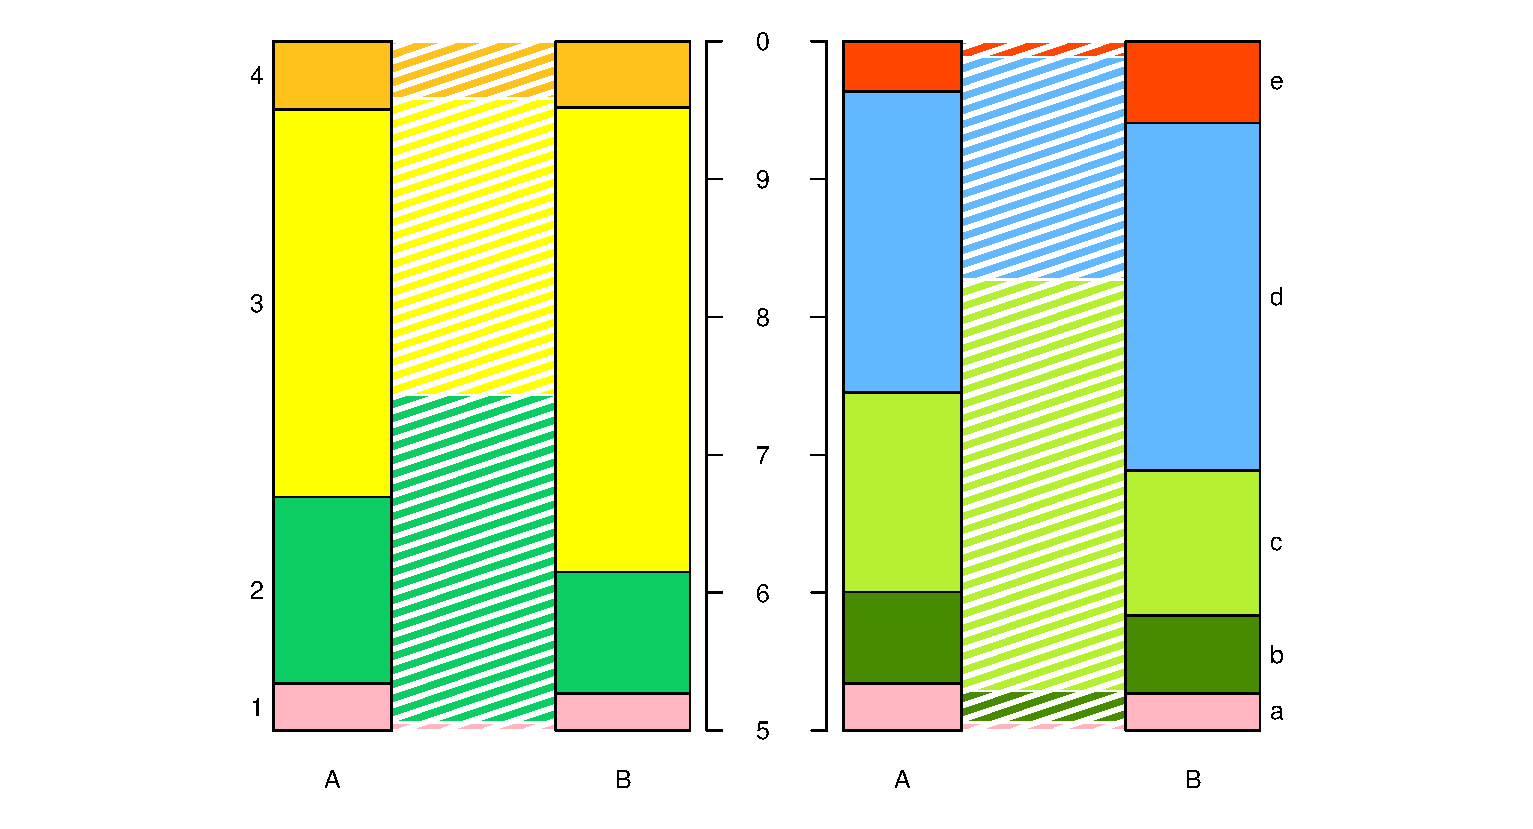
\includegraphics[width=7.425cm]{../figures/Nicaragua}}
\rput[bl](0.05,0.85) {\footnotesize Nicaragua (2005)}
%\psframe(0,0)(1,1)
}

%2,2
% 1,2
\rput[bl](1,1){
\rput[bl](0,0){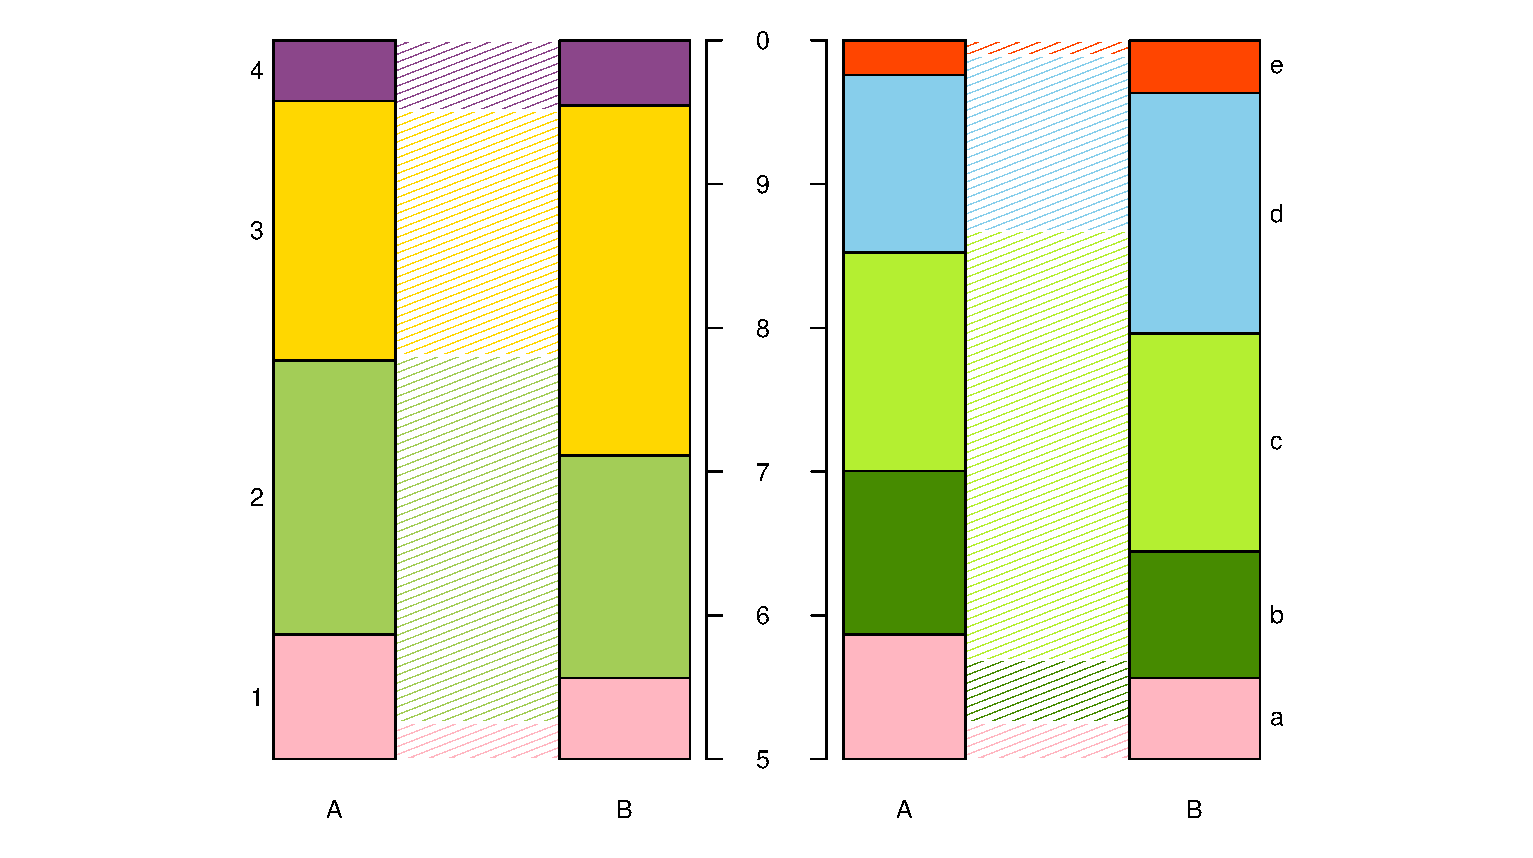
\includegraphics[width=7.425cm]{../figures/Panama}}
\rput[bl](0.05,0.85) {\footnotesize Panama (2010)}
%\psframe(0,0)(1,1)
}



\rput[bl](2,1){
\rput[bl](0,0){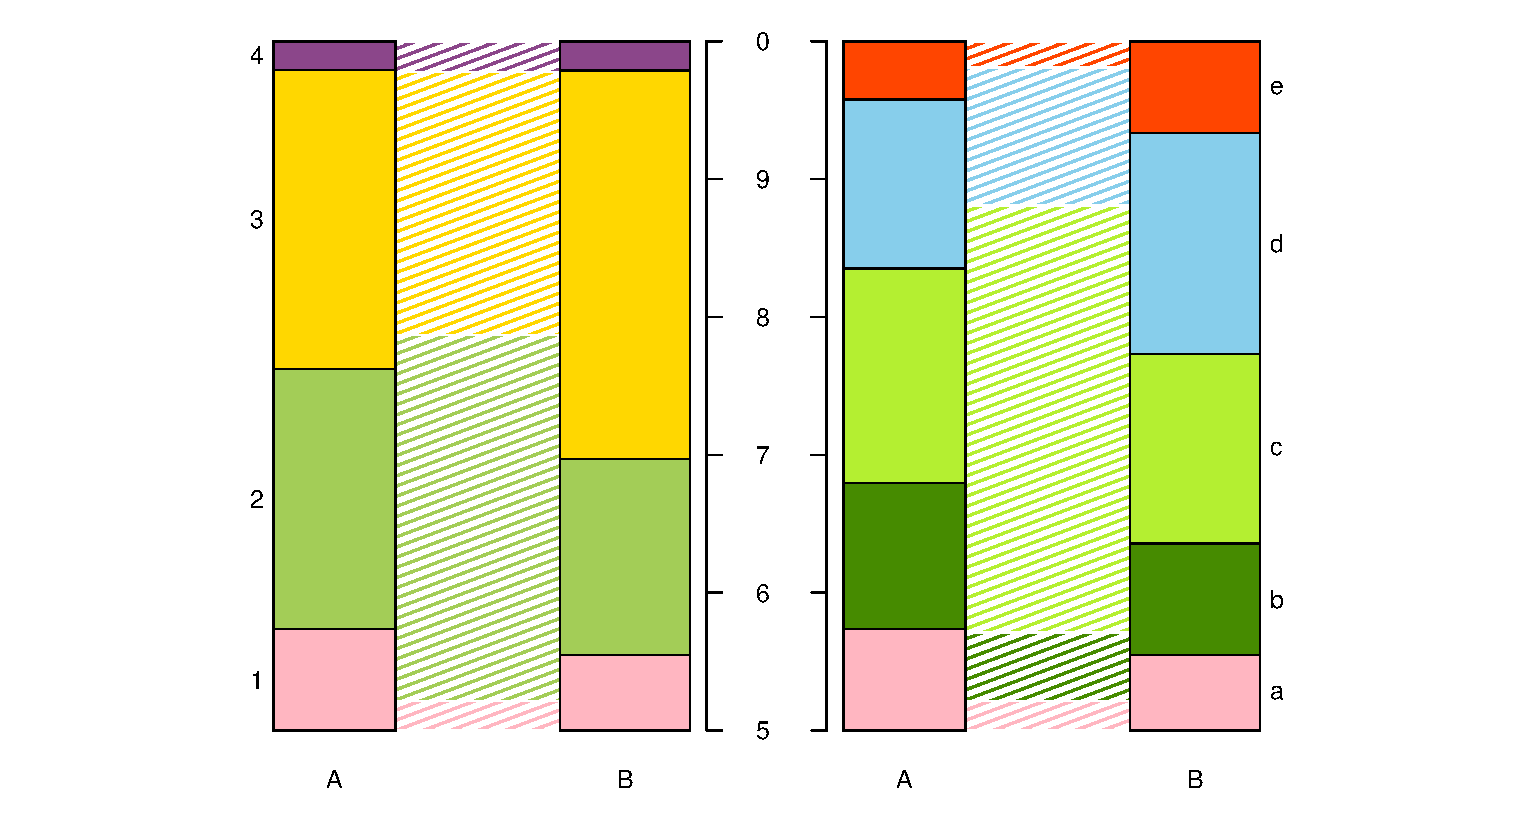
\includegraphics[width=7.425cm]{../figures/DominicanRepublic}}
\rput[bl](0.05,0.85) {\footnotesize Dominican Rep. (2010)}
%\psframe(0,0)(1,1)
}

\rput[bl](2,0){
\rput[bl](0,0){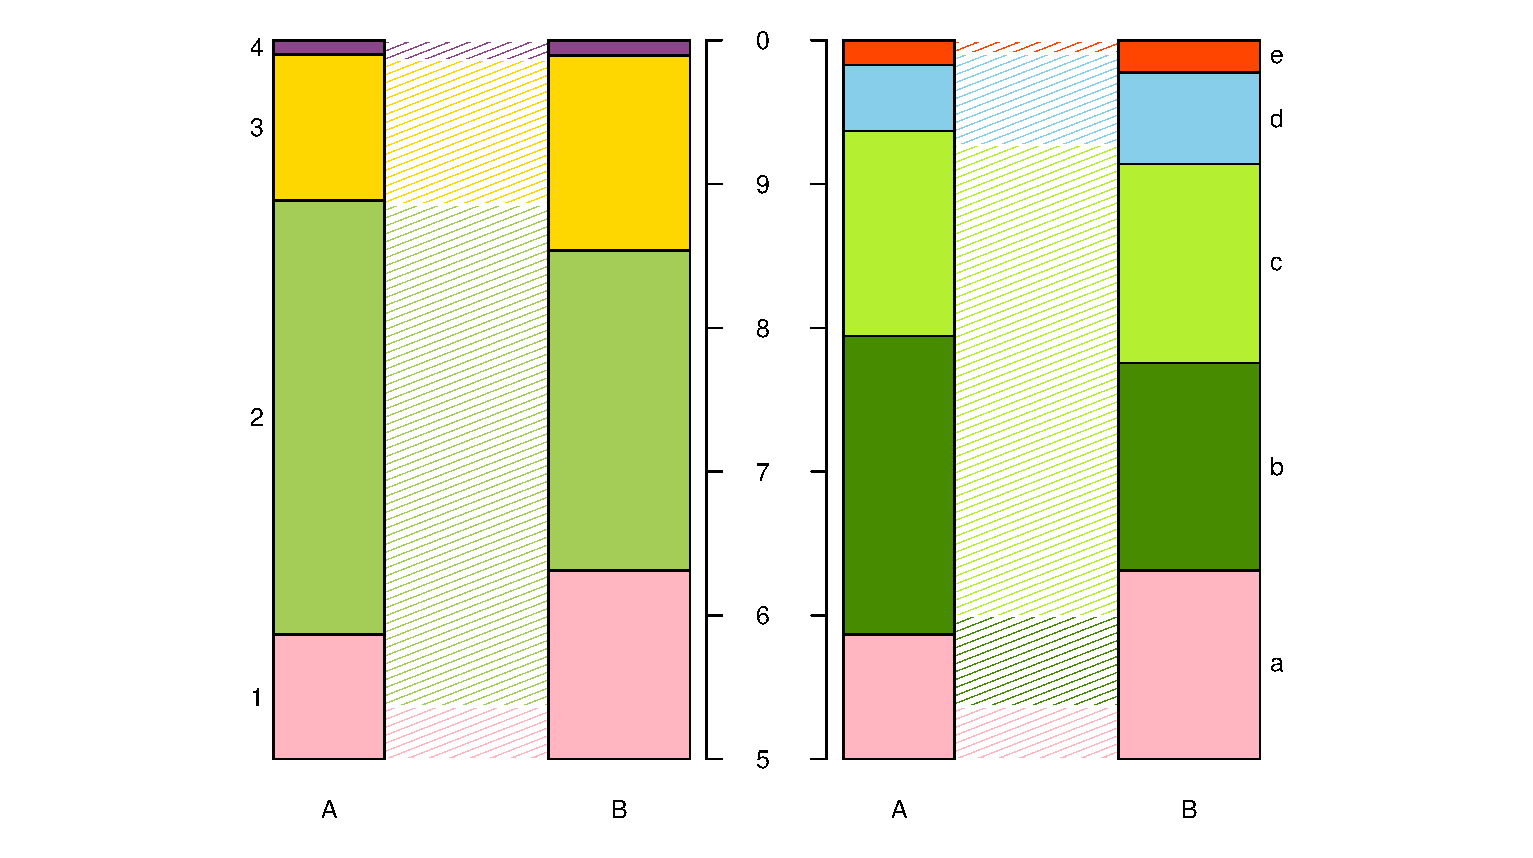
\includegraphics[width=7.425cm]{../figures/PuertoRico}}
\rput[bl](0.05,0.85) {\footnotesize Puerto Rico (2000)}
%\psframe(0,0)(1,1)
}

\rput[bl](3,1){
\rput[bl](0,0){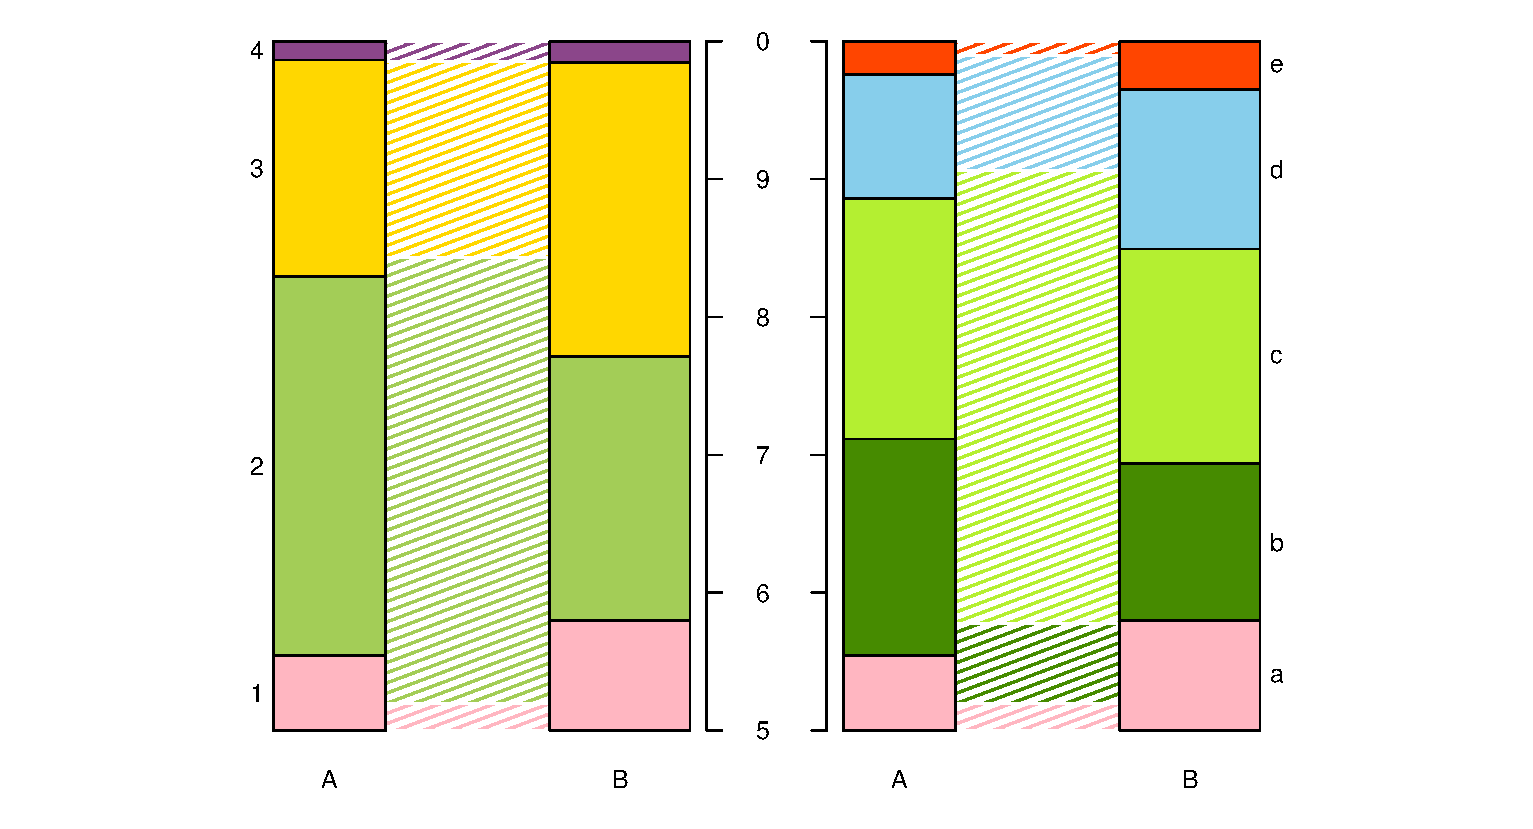
\includegraphics[width=7.425cm]{../figures/Brazil}}
\rput[bl](0.05,0.85) {\footnotesize Brazil (2010)}
%\psframe(0,0)(1,1)
}


\rput[bl](1,2.33){
\rput[bl](0,0){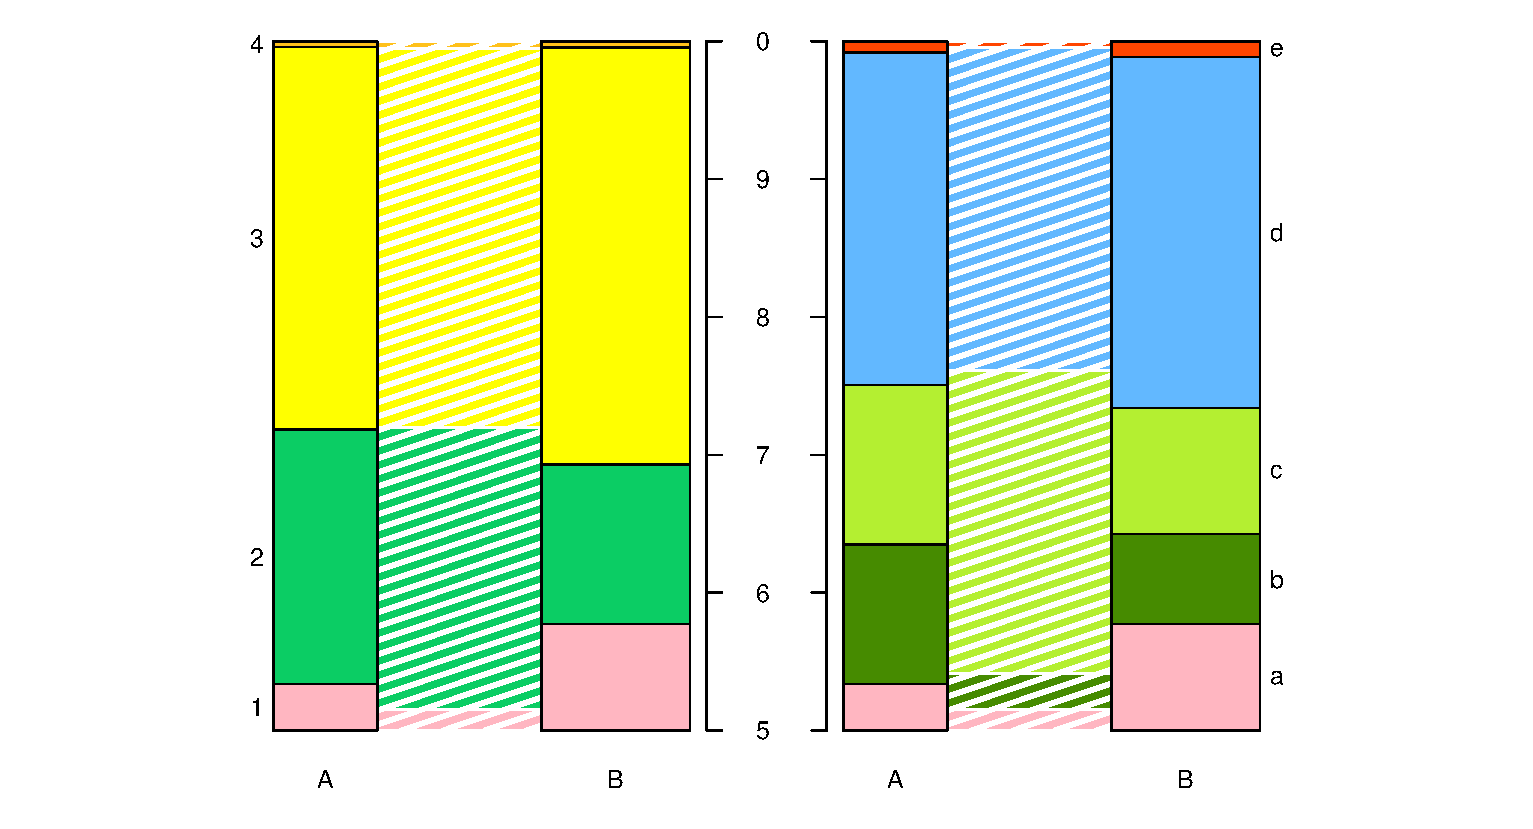
\includegraphics[width=7.425cm]{../figures/Armenia}}
\rput[bl](0.05,0.85) {\footnotesize Armenia (2011)}
%\psframe(0,0)(1,1)
} 
\rput[bl](3,2.33){
\rput[bl](0,0){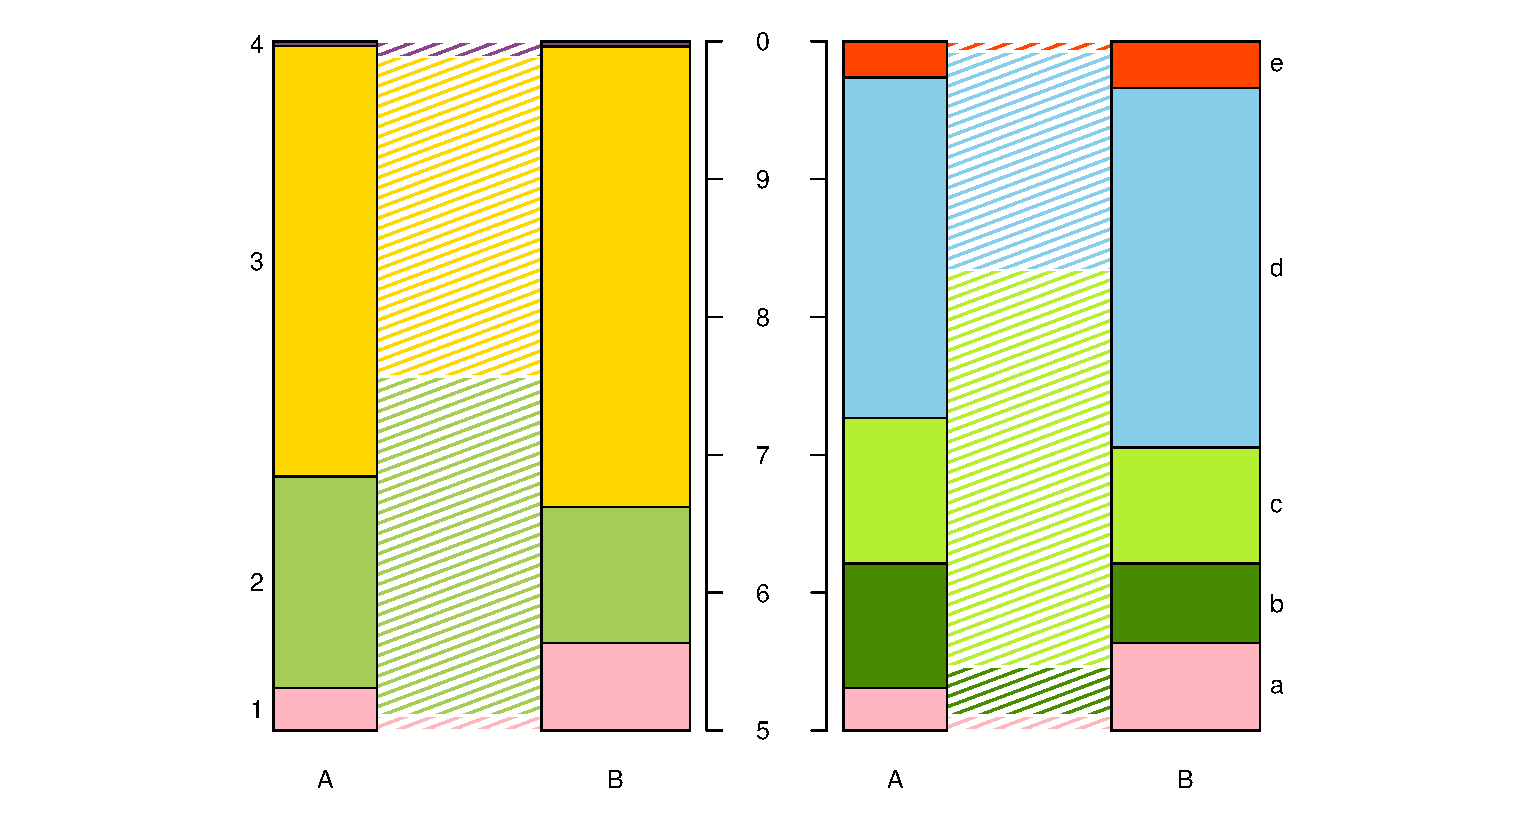
\includegraphics[width=7.425cm]{../figures/KyrgyzRepublic}}
\rput[bl](0.05,0.85) {\footnotesize Kyrgyz Republic (2009)}
%\psframe(0,0)(1,1)
} 
\rput[bl](2,2.33){
\rput[bl](0,0){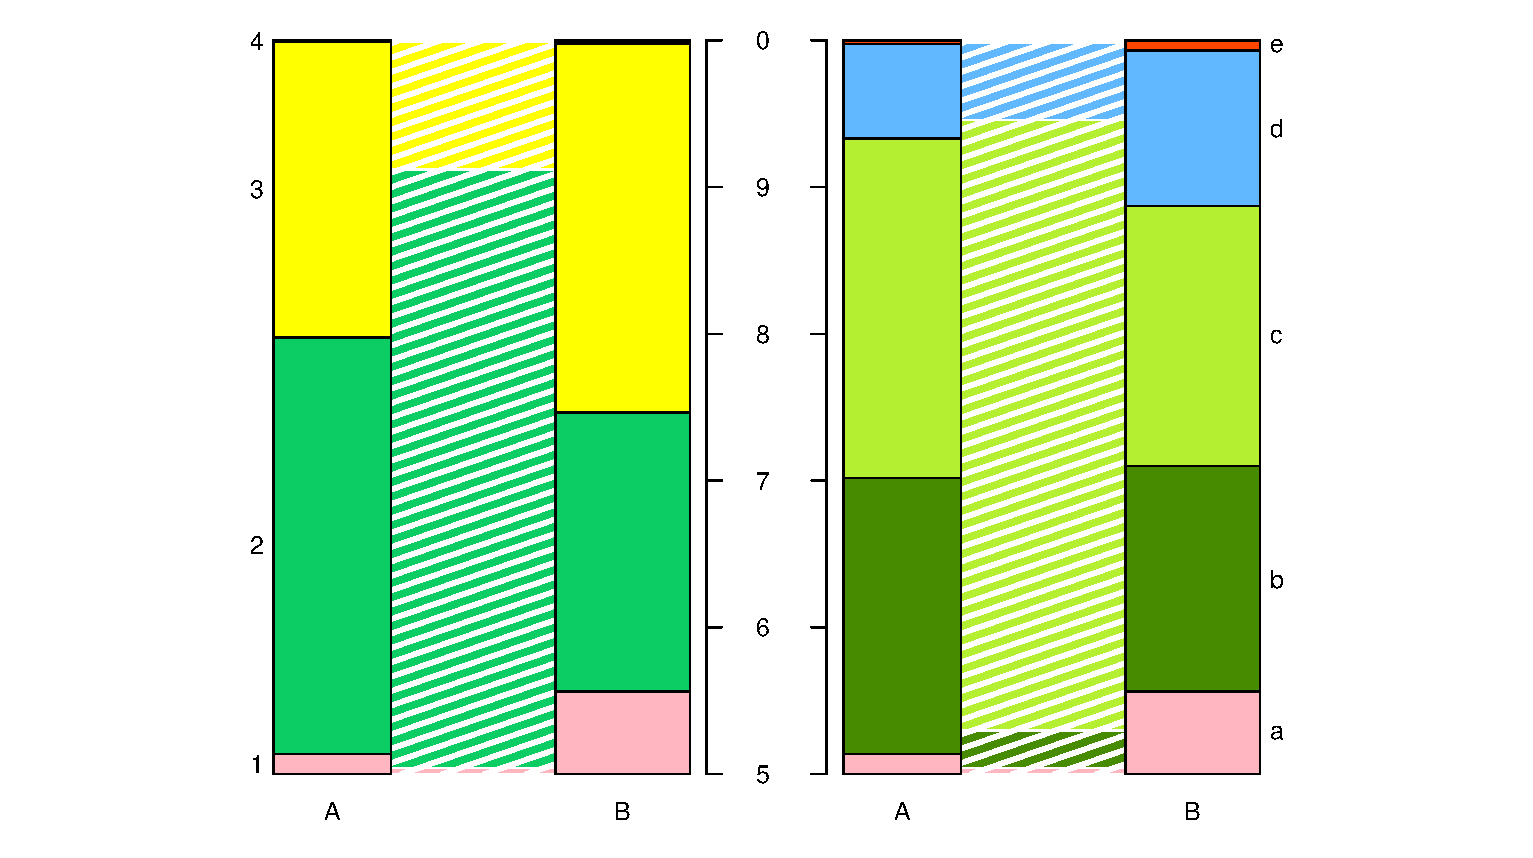
\includegraphics[width=7.425cm]{../figures/Palestine}}
\rput[bl](0.05,0.85) {\footnotesize Palestine (2009)}
%\psframe(0,0)(1,1)
} 

\rput[bl](2,3.33){
\rput[bl](0,0){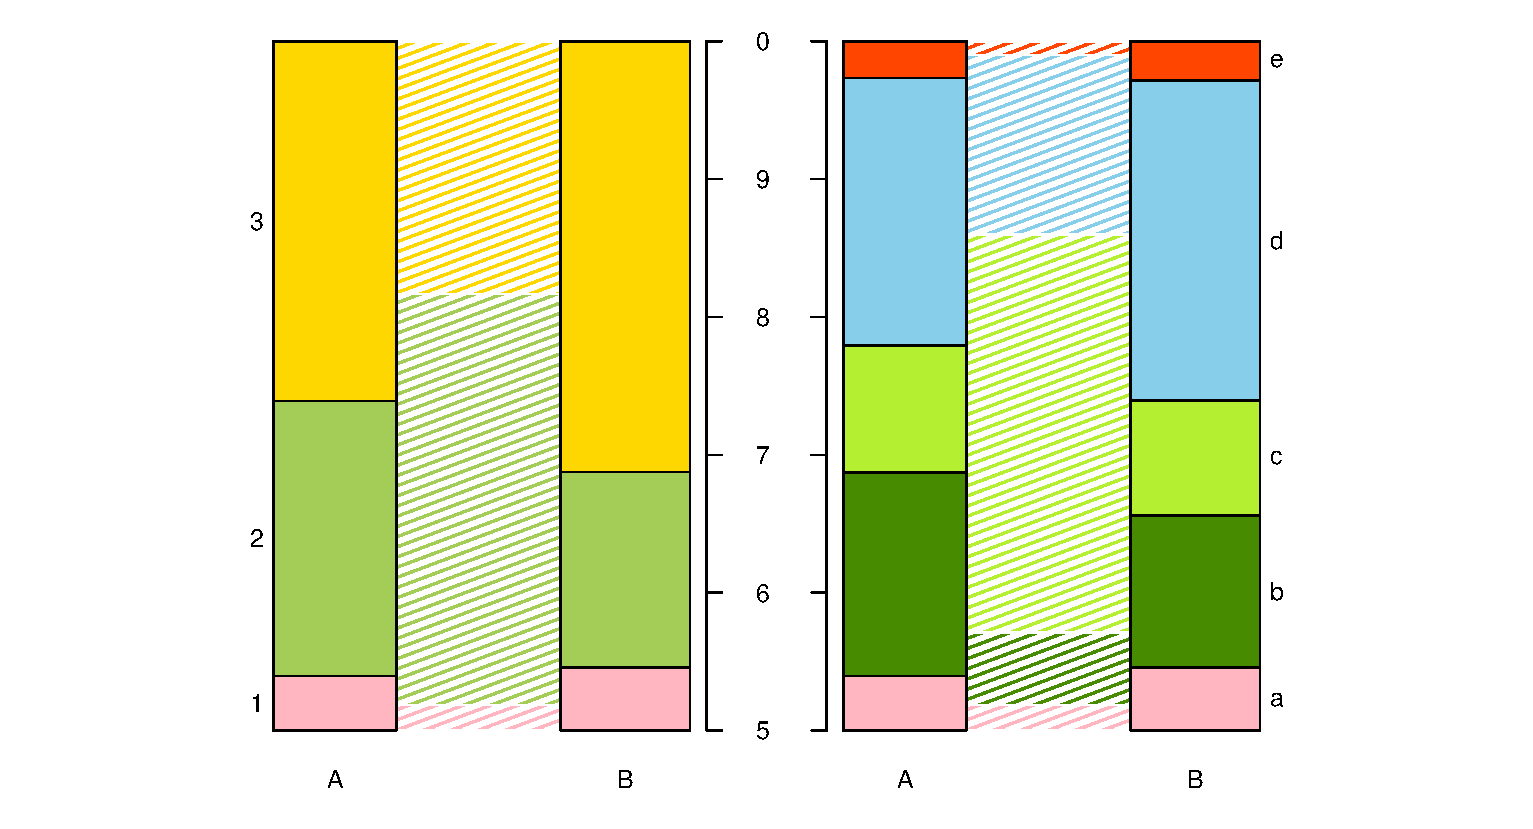
\includegraphics[width=7.425cm]{../figures/China}}
\rput[bl](0.05,0.85) {\footnotesize China (2000)}
%\psframe(0,0)(1,1)
} 

\rput[bl](3,3.33){
\rput[bl](0,0){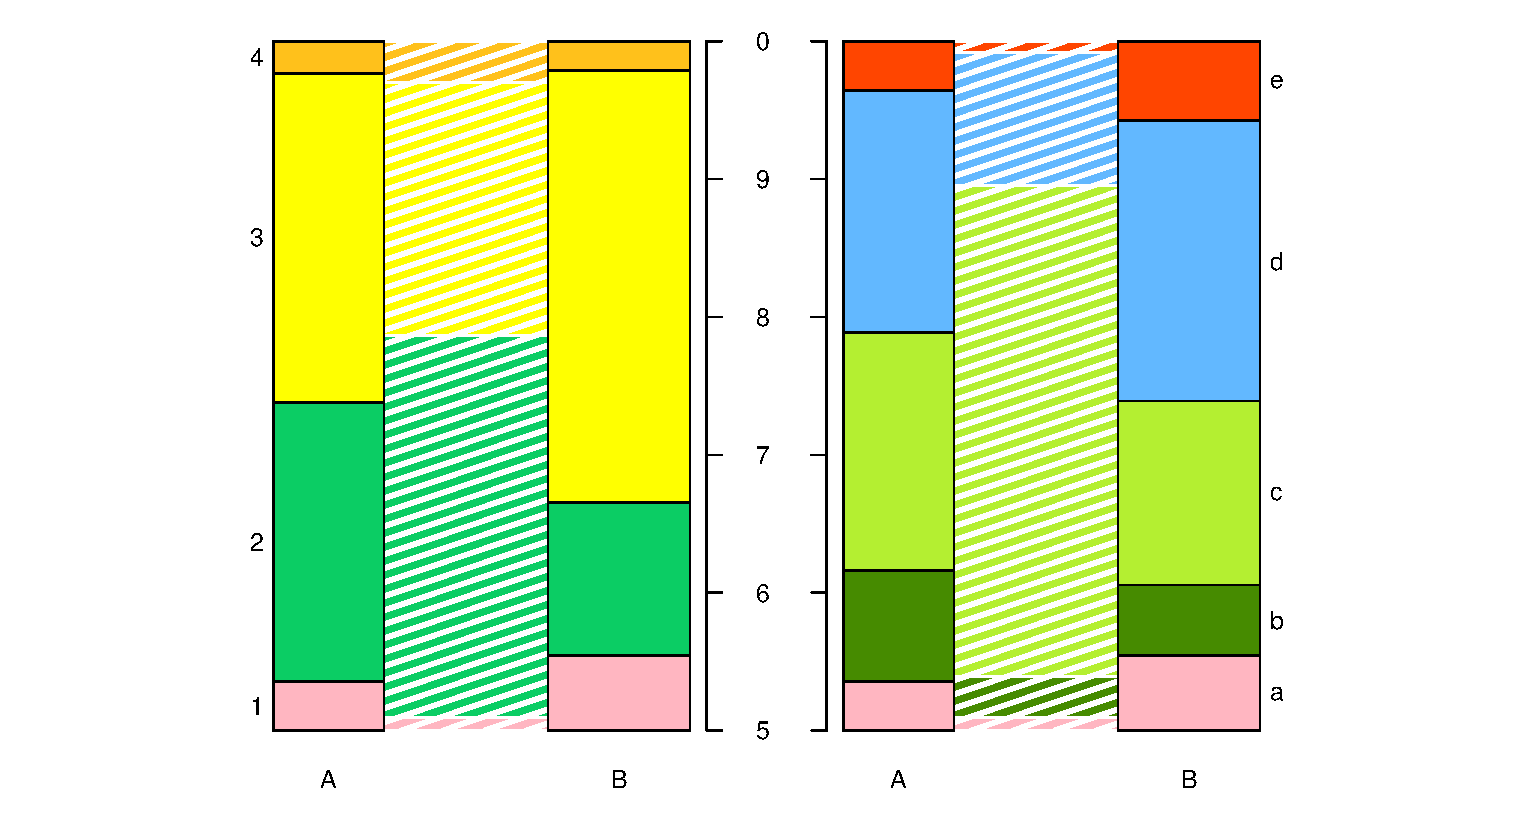
\includegraphics[width=7.425cm]{../figures/Mongolia}}
\rput[bl](0.05,0.85) {\footnotesize Mongolia (2000)}
%\psframe(0,0)(1,1)
} 
\rput[bl](2.05,4.43){\large \textsc{Asia}
}

\rput[bl](3,4.66){
\rput[bl](0,0){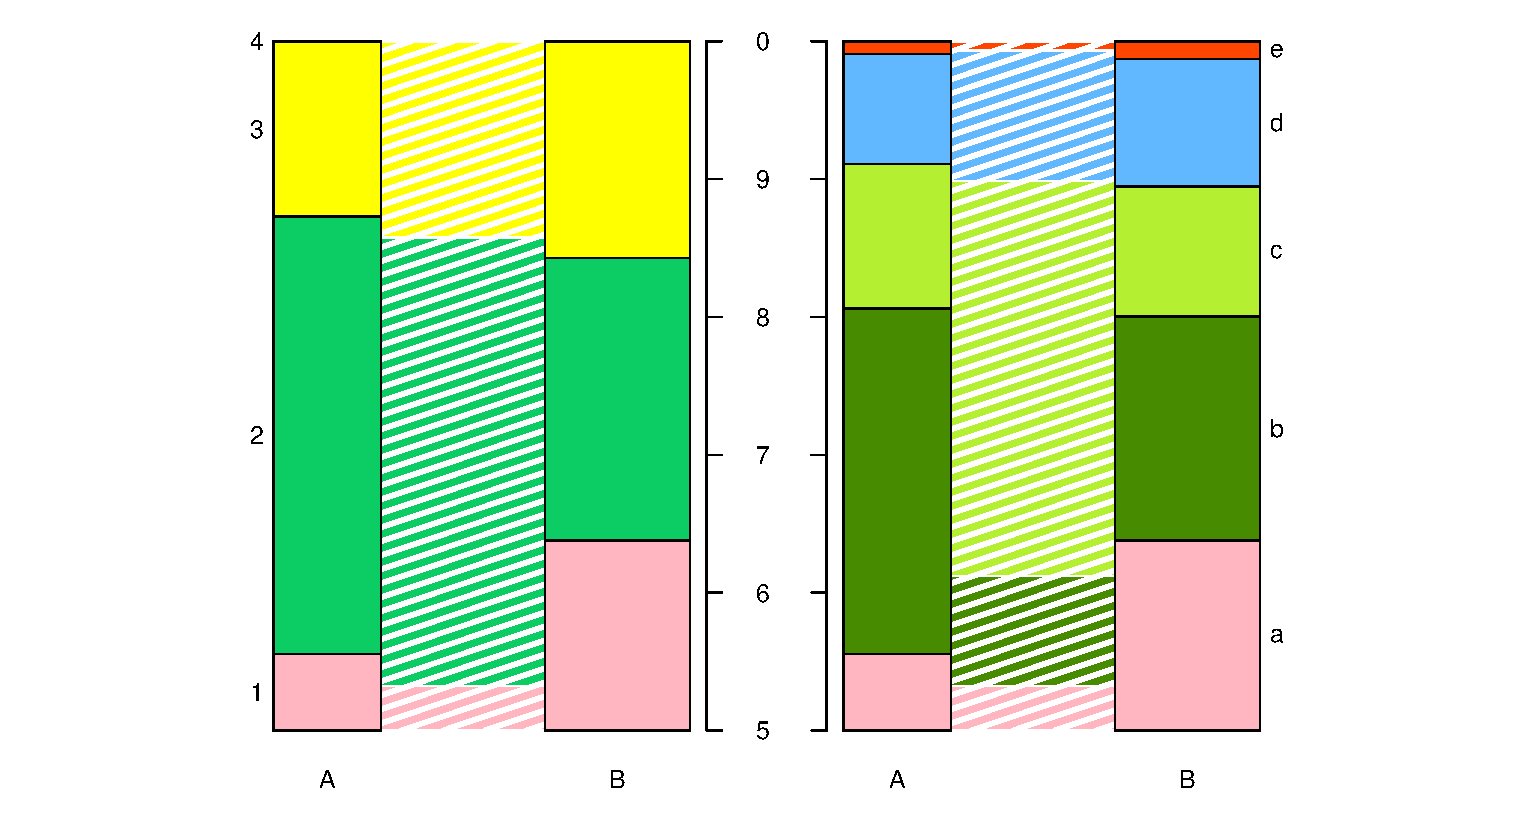
\includegraphics[width=7.425cm]{../figures/Romania}}
\rput[bl](0.05,0.85) {\footnotesize Romania (2011)}
%\psframe(0,0)(1,1)
} 

\rput[bl](2,4.66){
\rput[bl](0,0){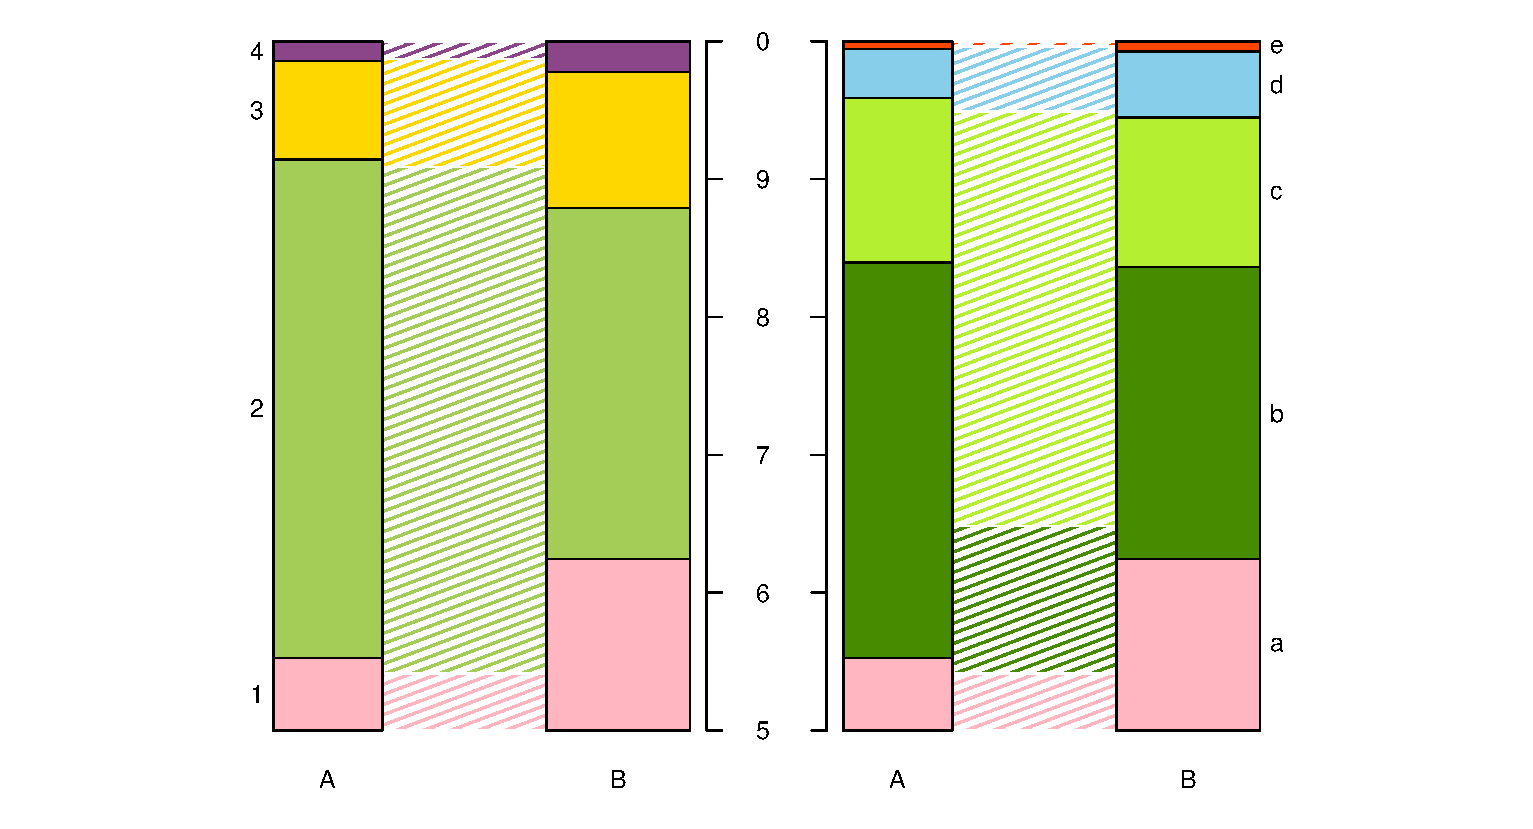
\includegraphics[width=7.425cm]{../figures/Portugal}}
\rput[bl](0.05,0.85) {\footnotesize Portugal (2011)}
%\psframe(0,0)(1,1)
} 
\rput[bl](3,5.66){
\rput[bl](0,0){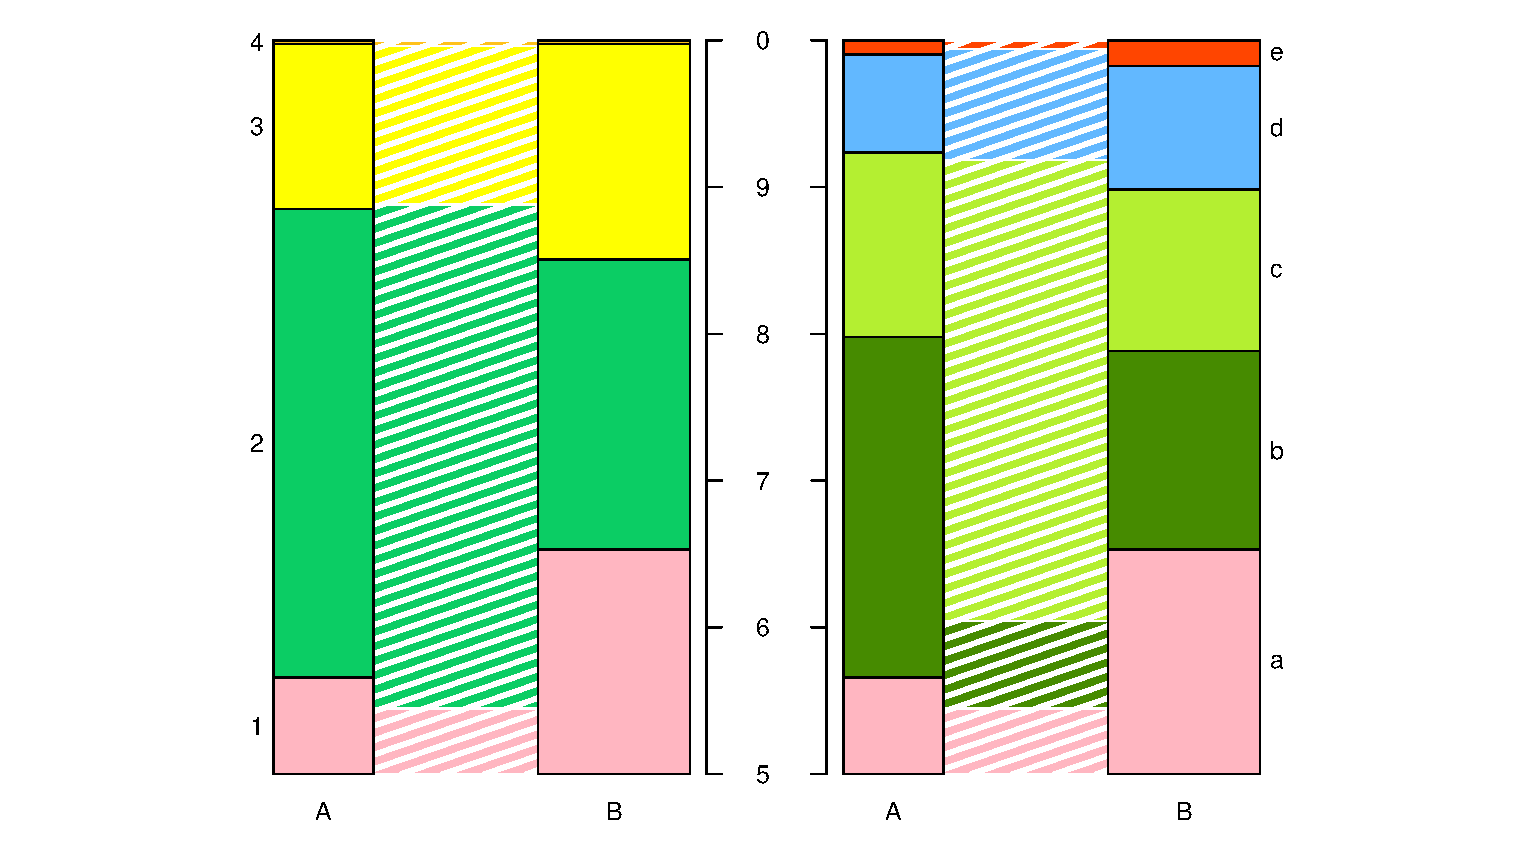
\includegraphics[width=7.425cm]{../figures/Poland}}
\rput[bl](0.05,0.85) {\footnotesize Poland (2011)}
%\psframe(0,0)(1,1)
} 
\rput[bl](3,6.66){
\rput[bl](0,0){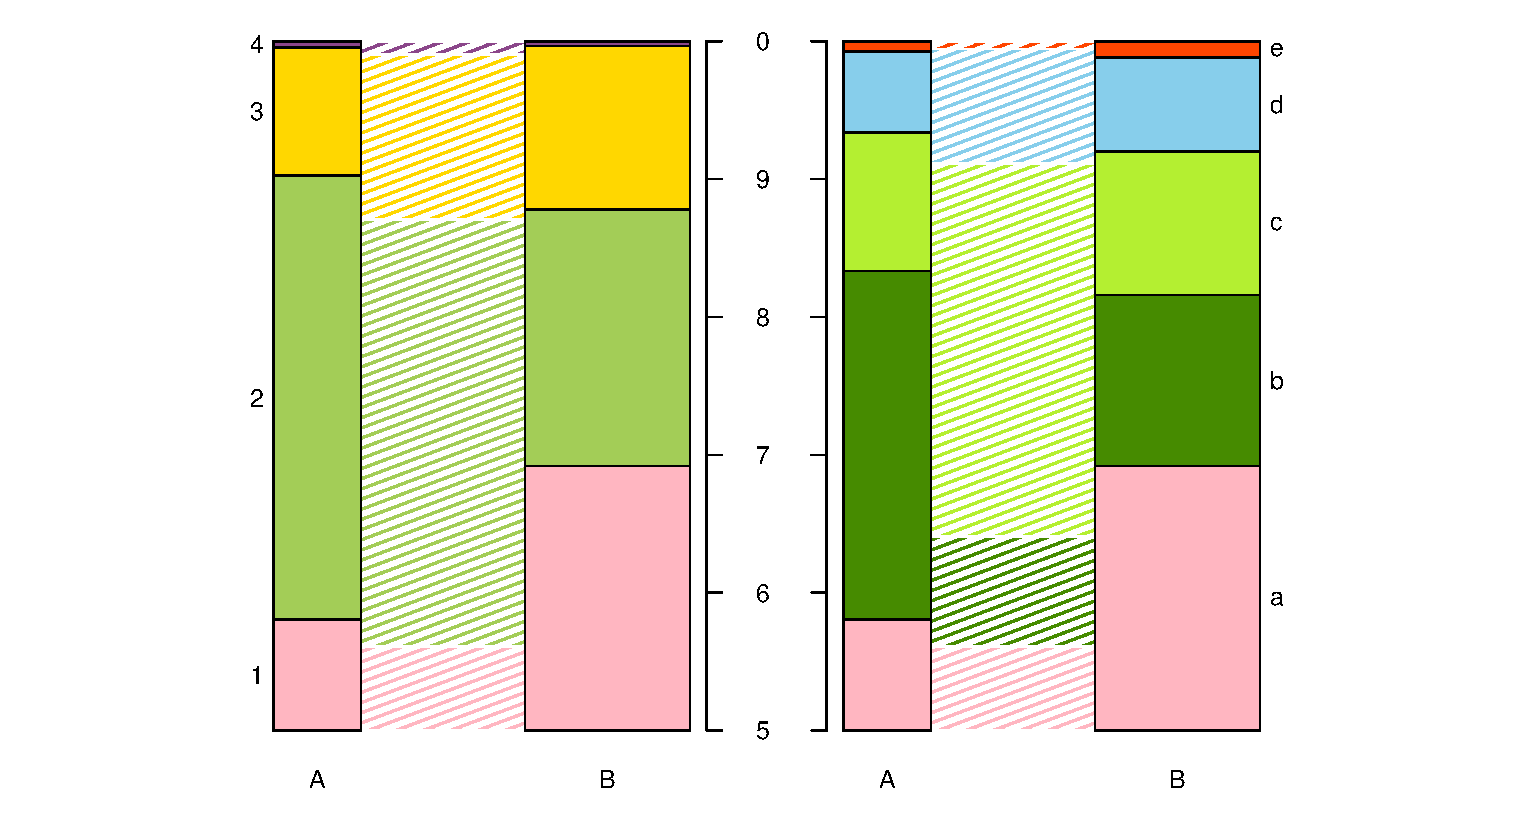
\includegraphics[width=7.425cm]{../figures/Belarus}}
\rput[bl](0.05,0.85) {\footnotesize Belarus (2011)}
%\psframe(0,0)(1,1)
} 

\rput[bl](2,5.66){
\rput[bl](0,0){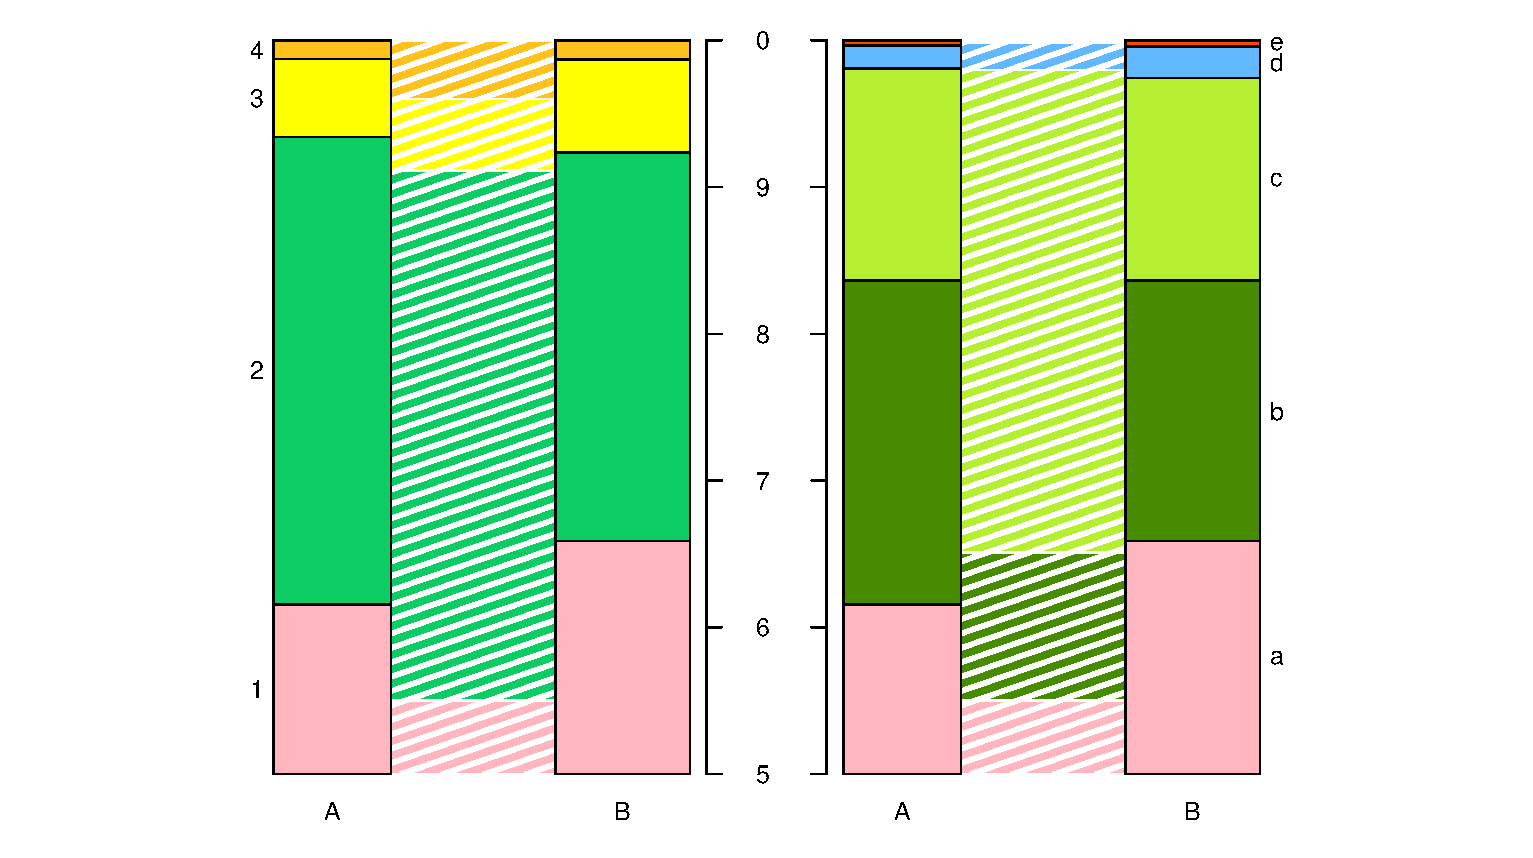
\includegraphics[width=7.425cm]{../figures/Ireland}}
\rput[bl](0.05,0.85) {\footnotesize Ireland (2011)}
%\psframe(0,0)(1,1)
} 

\rput[bl](2.05,7.76){\large \textsc{Europe}
}

\rput[bl](2,6.66){
\rput[bl](0,0){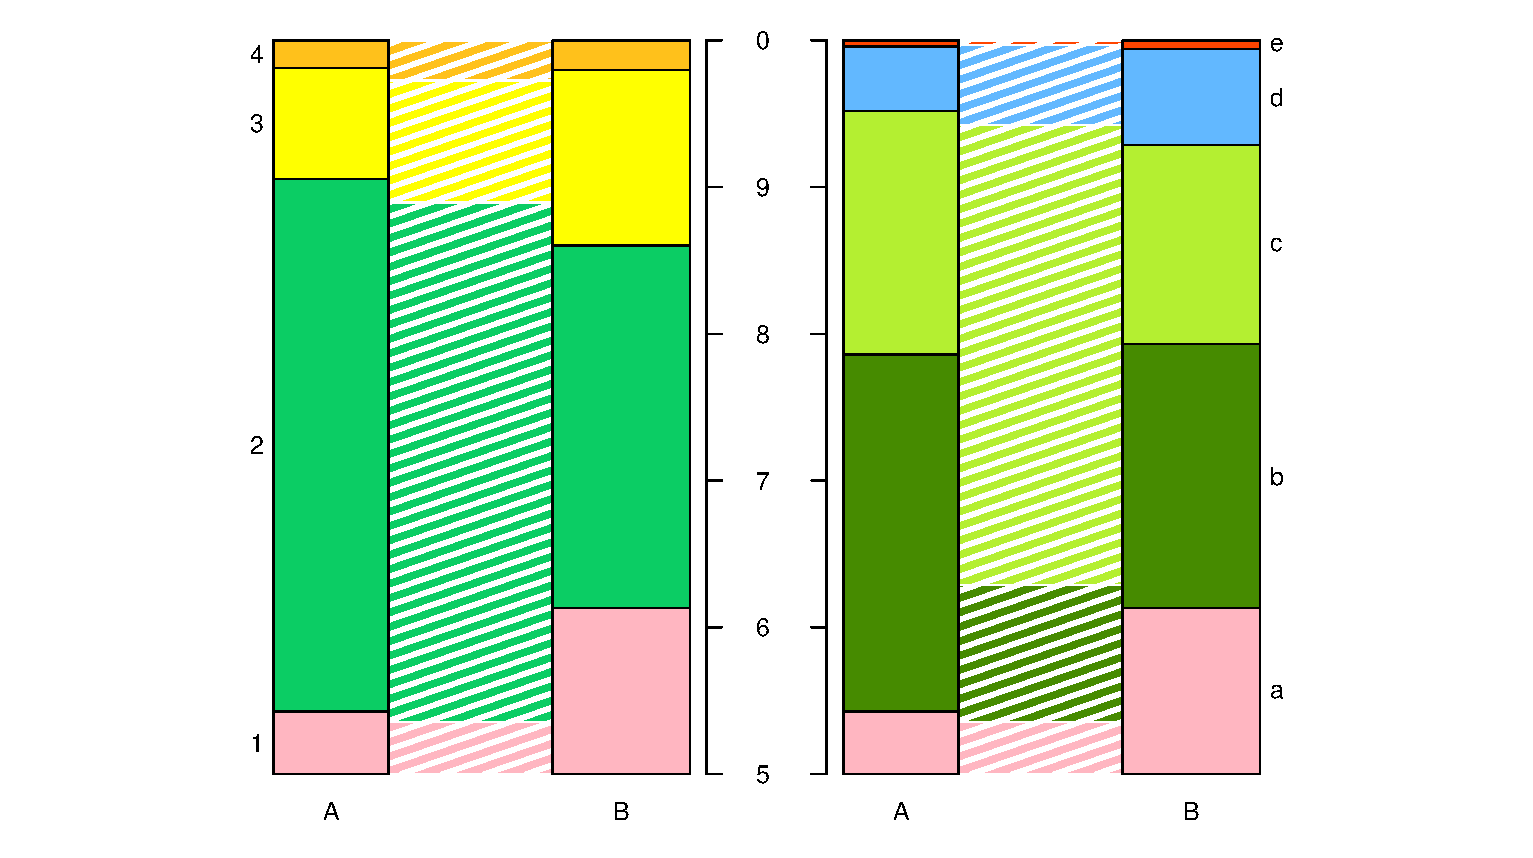
\includegraphics[width=7.425cm]{../figures/Greece}}
\rput[bl](0.05,0.85) {\footnotesize Greece (2011)}
%\psframe(0,0)(1,1)
} 

\rput[bl](0.05,6.43){\large \textsc{Africa}
}
\rput[bl](0,5.33){
\rput[bl](0,0){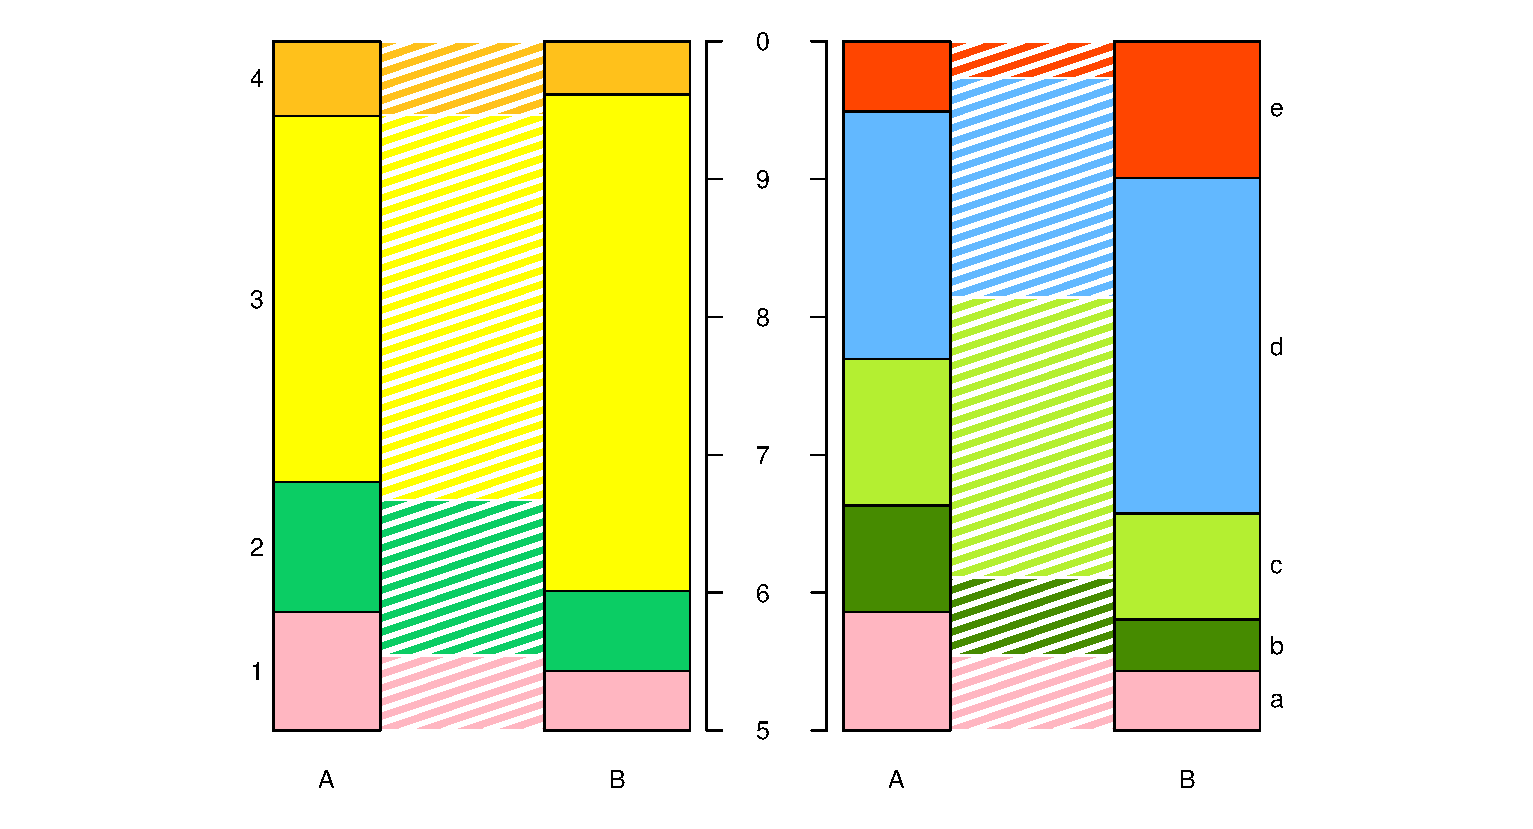
\includegraphics[width=7.425cm]{../figures/Botswana}}
\rput[bl](0.05,0.85) {\footnotesize Botswana (2011)}
%\psframe(0,0)(1,1)
} 
\rput[bl](1,5.33){
\rput[bl](0,0){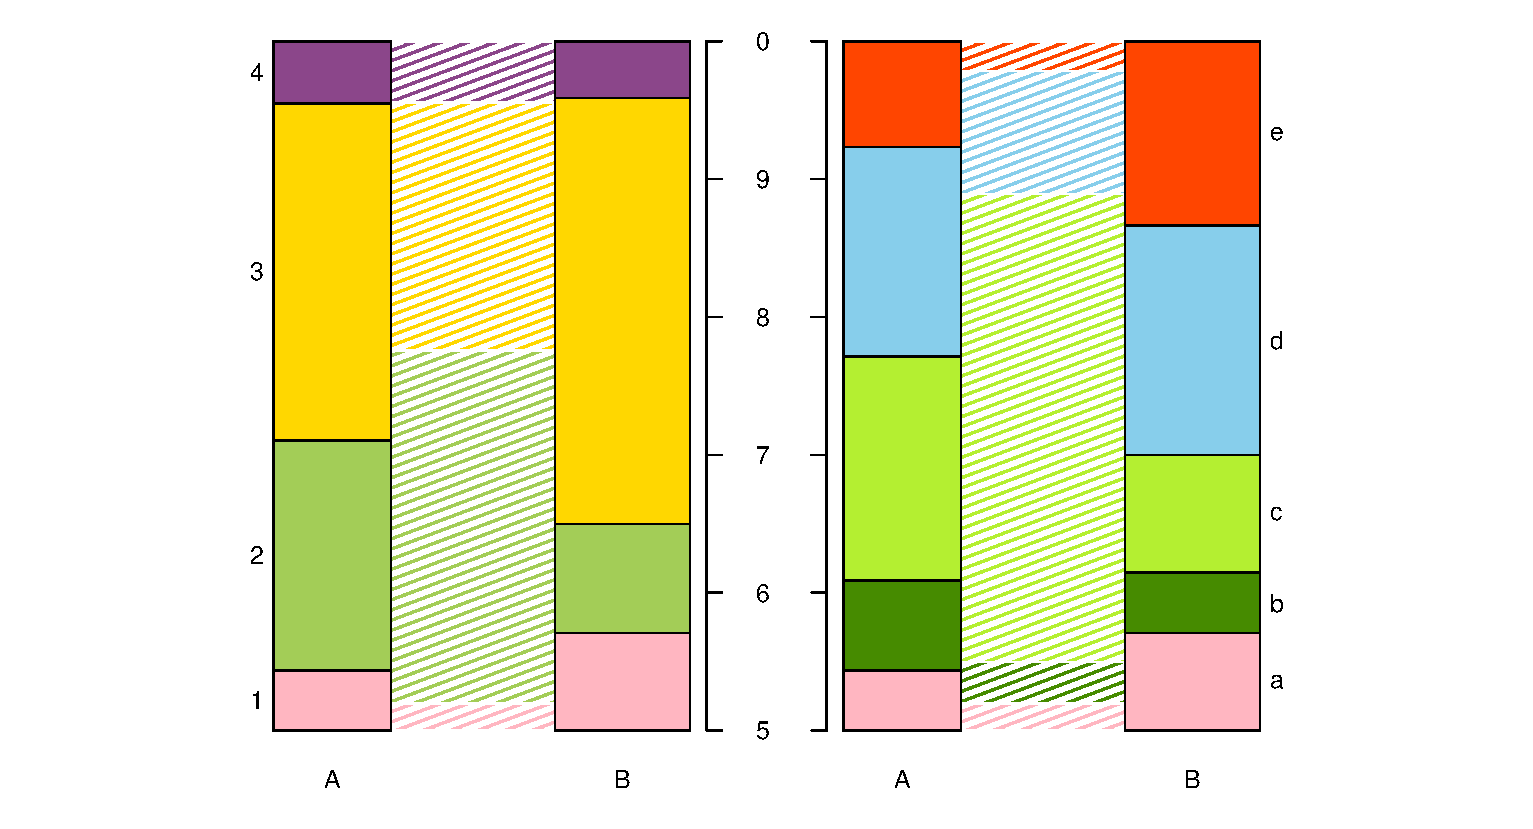
\includegraphics[width=7.425cm]{../figures/Kenya}}
\rput[bl](0.05,0.85) {\footnotesize Kenya (2011)}
%\psframe(0,0)(1,1)
} 

\rput[bl](0,4.33){
\rput[bl](0,0){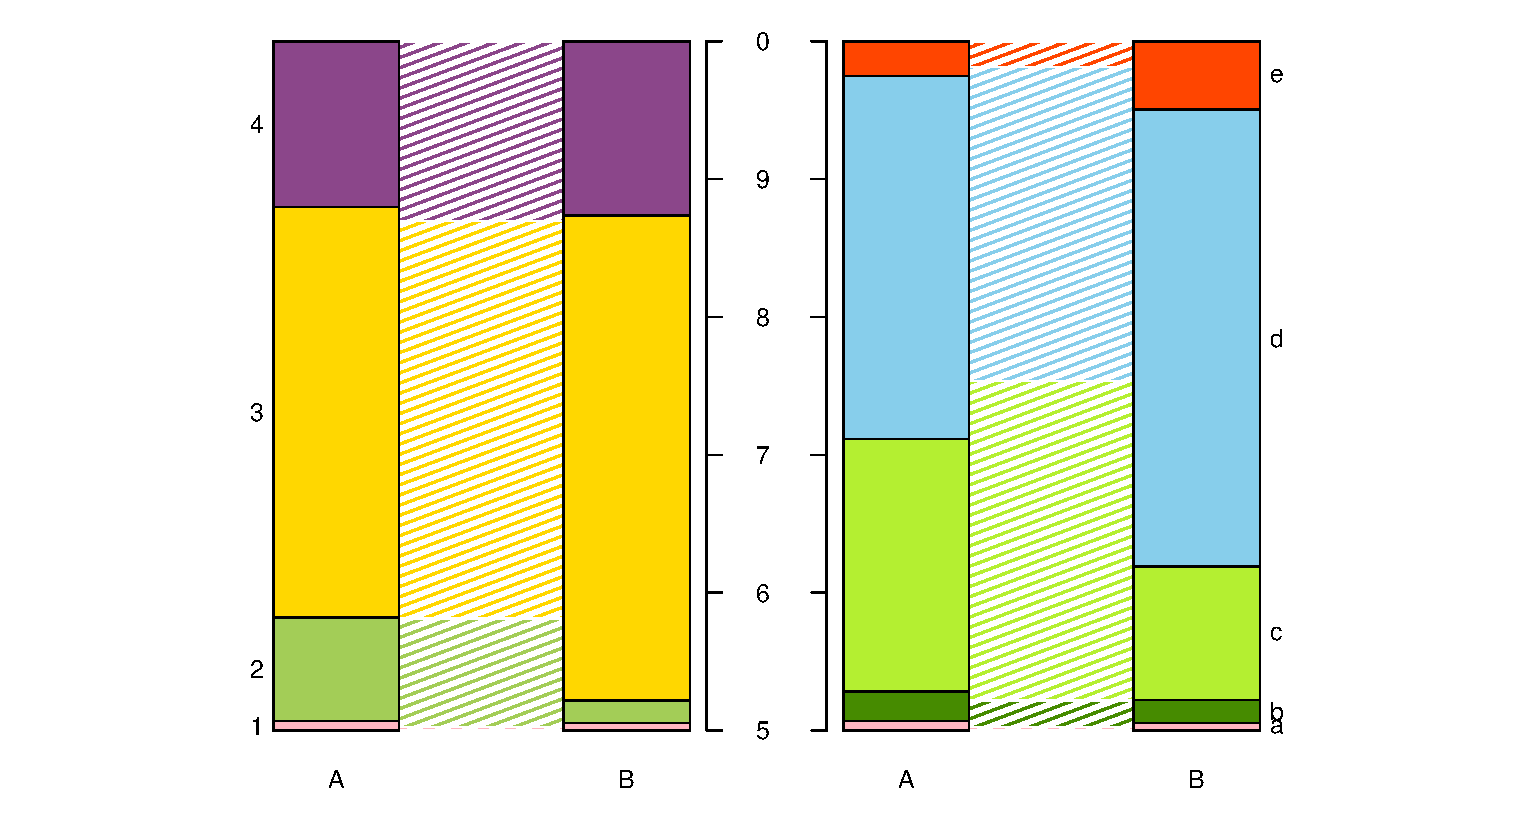
\includegraphics[width=7.425cm]{../figures/Senegal}}
\rput[bl](0.05,0.85) {\footnotesize Senegal (2011)}
%\psframe(0,0)(1,1)
} 

\rput[bl](1,4.33){
\rput[bl](0,0){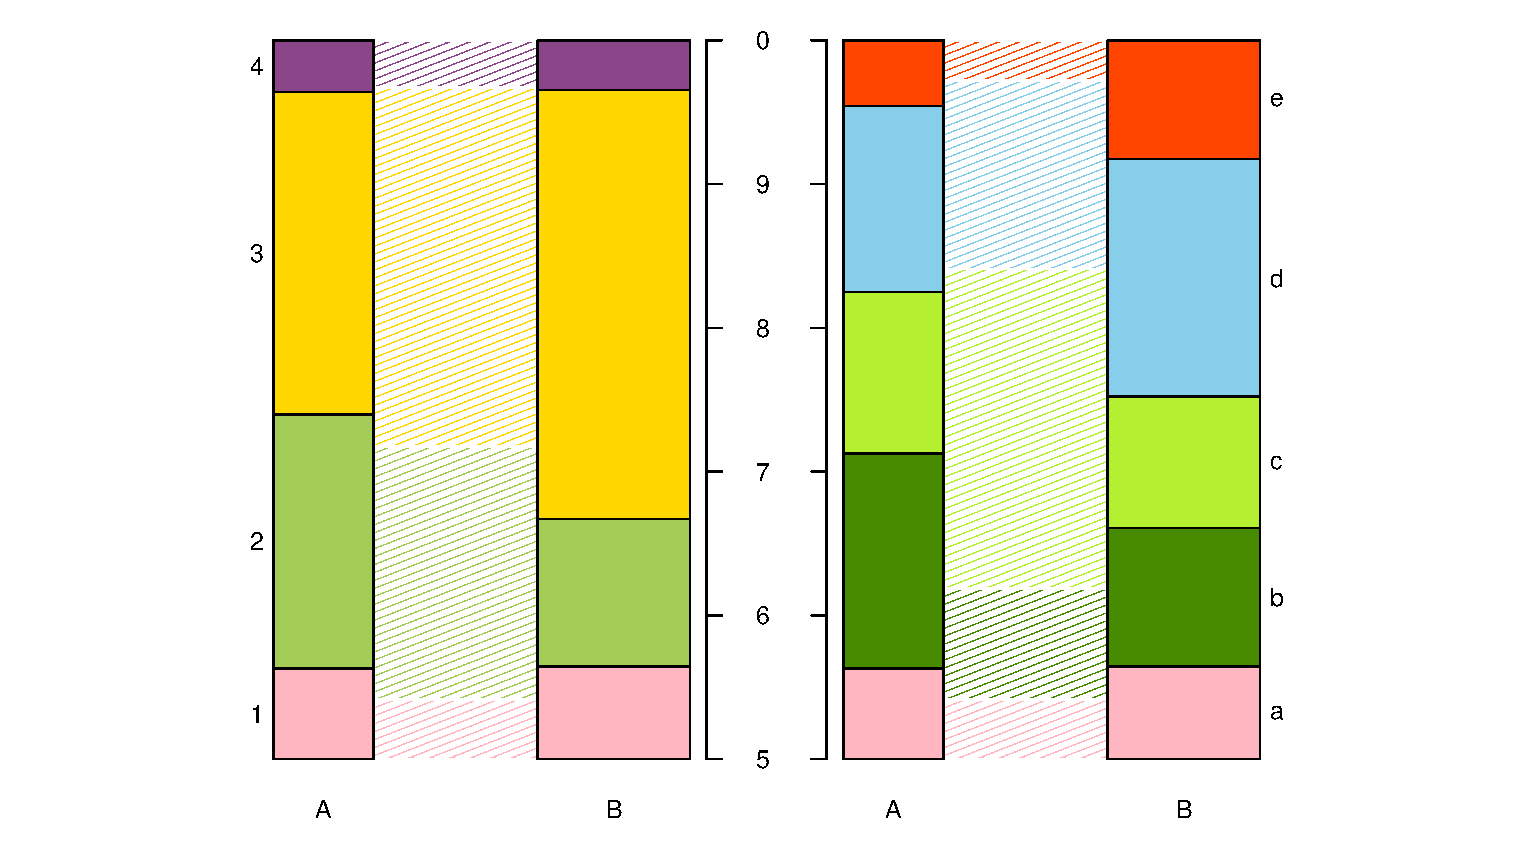
\includegraphics[width=7.425cm]{../figures/SouthAfrica}}
\rput[bl](0.05,0.85) {\footnotesize SouthAfrica (2011)}
%\psframe(0,0)(1,1)
} 

 }

\psset{xunit=1cm, yunit=1cm}


%
%\rput[br](20,24.5){
%\rput[br](0,0.2){
%\mini{\parbox[c]
%{4.5cm}{\mini *The four former Soviet republics shown on the right became independent in 1991; however their government's population policies are first recorded only in the 1996 UN report, hence the narrower charts. 
%}}}
%}
%
%% Arab
%\rput[tl](0,9.94){
%% 3,1
%\rput[tl](0,26.066667){\includegraphics[width=7.425cm]{figures/iran}}
%\rput[tl](0.5, 26.566667) {\footnotesize  Iran}
%% 3,2
%\rput[tl](7.425,26.066667){\includegraphics[width=7.425cm]{figures/kuwait}}
%\rput[tl](7.925,26.566667) {\footnotesize  Kuwait}
%% 4,1
%\rput[tl](0,21.093333){\includegraphics[width=7.425cm]{figures/qatar}}
%\rput[tl](0.5, 21.593333) {\small  Qatar}
%% 4,2
%\rput[tl](7.425,21.093333){\includegraphics[width=7.425cm]{figures/saudi.arabia}}
%\rput[tl](7.925, 21.593333) {\footnotesize  Saudi Arabia}
%% 5,1
%\rput[tl](0,16.120000 ){\includegraphics[width=7.425cm]{figures/turkey}}
%\rput[tl](0.5,  16.620000) {\footnotesize  Turkey}
%% 5,2
%\rput[tl](7.425,16.120000 ){\includegraphics[width=7.425cm]{figures/uae}}
%\rput[tl](7.925,  16.620000) {\footnotesize  United Arab Emirates}
%}
%
%
%% ASIA
%\rput[tl](0,7.46){
%% 5,3
%\rput[tl](14.85,16.120000 ){\includegraphics[width=7.425cm]{figures/china}}
%\rput[tl](15.35,  16.620000) {\footnotesize China}
%% 5,4
%\rput[tl](22.275,16.120000 ){\includegraphics[width=7.425cm]{figures/dprk}}
%\rput[tl](22.775,  16.620000) {\footnotesize  DPR Korea}
%% 6,3
%\rput[tl](14.85,11.146667){\includegraphics[width=7.425cm]{figures/mongolia}}
%\rput[tl](15.35,11.646667) {\footnotesize Mongolia}
%% 6,4
%\rput[tl](22.275,11.146667){\includegraphics[width=7.425cm]{figures/korea}}
%\rput[tl](22.775, 11.646667) {\footnotesize  Republic of Korea}
%% 7,3
%\rput[tl](14.85,6.173333){\includegraphics[width=7.425cm]{figures/singapore}}
%\rput[tl](15.35,6.673333) {\footnotesize Singapore}
%% 7,4
%\rput[tl](22.275,6.173333){\includegraphics[width=7.425cm]{figures/thailand}}
%\rput[tl](22.775, 6.673333) {\small  Thailand}
%}
%
%% MEd
%\rput[tl](0,4.973333){
%% 7,1
%\rput[tl](0,6.173333){\includegraphics[width=7.425cm]{figures/cyprus}}
%\rput[tl](0.5,6.673333) {\small Cyprus}
%% 7,2
%\rput[tl](7.425,6.173333){\includegraphics[width=7.425cm]{figures/israel}}
%\rput[tl](7.925, 6.673333) {\small  Israel}
%}
%
%% afr
%\rput[tl](0,7.46){
%% 7,1
%\rput[tl](0,11.146667){\includegraphics[width=7.425cm]{figures/gabon}}
%\rput[tl](0.5, 11.646667) {\small Gabon}
%% 7,2
%\rput[tl](7.425,11.146667){\includegraphics[width=7.425cm]{figures/mauritius}}
%\rput[tl](7.925,  11.646667) {\small  Mauritius}
%}

\end{pspicture}


\end{document}



